\usetikzlibrary{calc}
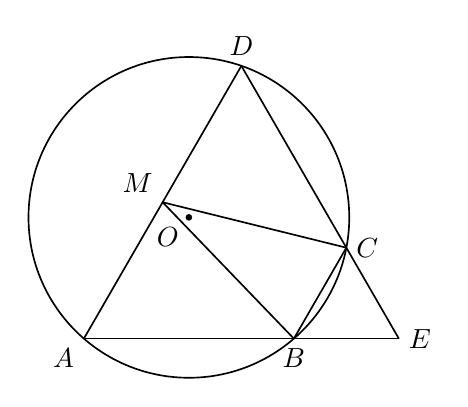
\begin{tikzpicture}[x=1cm,y=1cm,line width=.6pt,font=\normalsize]
\coordinate (A) at (0,0);
\coordinate (E) at (4,0);
\coordinate (D) at (2,3.464102);
\coordinate (B) at (2.666667,0);
\coordinate (C) at (3.333333,1.154701);
\coordinate (M) at (1,1.732051);
\coordinate (O) at (1.333333,1.539601);
\draw (O) circle[radius=2.0367cm];
\draw (A)--(E);
\draw (A)--(D);
\draw (D)--(E);
\draw (B)--(C);
\draw (M)--(B);
\draw (M)--(C);
\fill (O) circle[radius=1.2pt];
\node[below left] at (A) {$A$};
\node[right] at (E) {$E$};
\node[above] at (D) {$D$};
\node[below] at (B) {$B$};
\node[right] at (C) {$C$};
\node[above left] at (M) {$M$};
\node[below left] at (O) {$O$};
\end{tikzpicture}
